\chapter{Развертывание кластера}

\section{Конфигурирование узлов гипервизора}

\subsection{Первоначальная настройка управляющего узла}

Первым делом создадим управляющий узел кластера. Этот процесс отображен на рисунках \ref{init/01} -- \ref{init/10}

\begin{figure}[H]
	\centering
	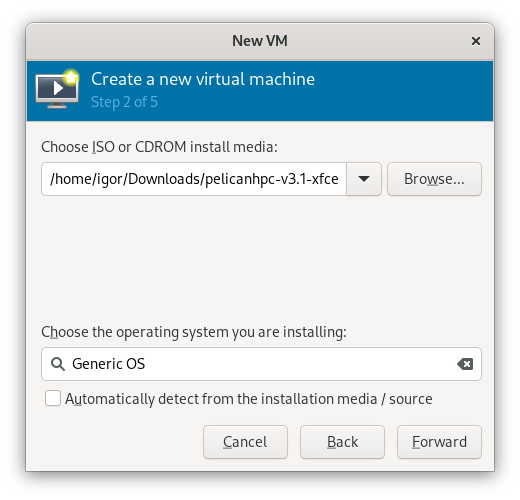
\includegraphics[width=0.5\linewidth]{1-01}
	\caption{Выбор образа ОС}
	\label{init/01}
\end{figure}

\begin{figure}[H]
	\centering
	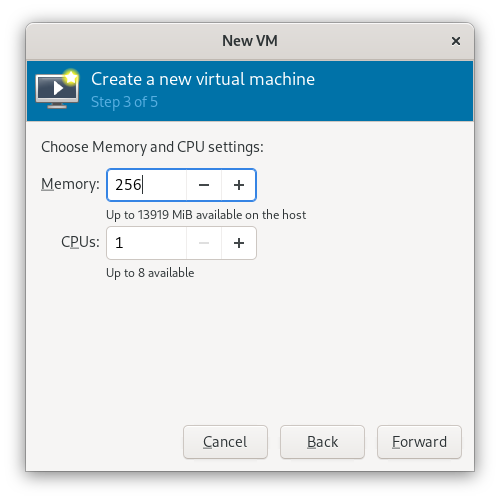
\includegraphics[width=0.5\linewidth]{1-02}
	\caption{Выделение ресурсов управляющему узлу}
	\label{init/02}
\end{figure}

\begin{figure}[H]
	\centering
	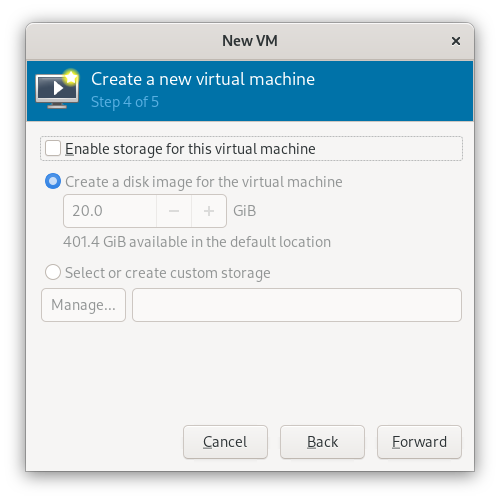
\includegraphics[width=0.5\linewidth]{1-03}
	\caption{Отключение дискового хранилища ВМ}
	\label{init/03}
\end{figure}

\begin{figure}[H]
	\centering
	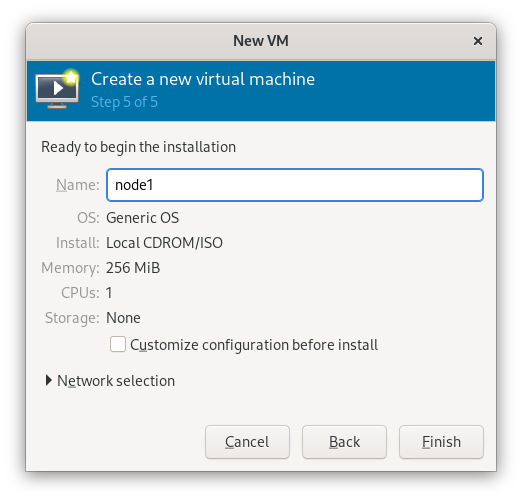
\includegraphics[width=0.5\linewidth]{1-04}
	\caption{Выбор имени ВМ}
	\label{init/04}
\end{figure}

\begin{figure}[H]
	\centering
	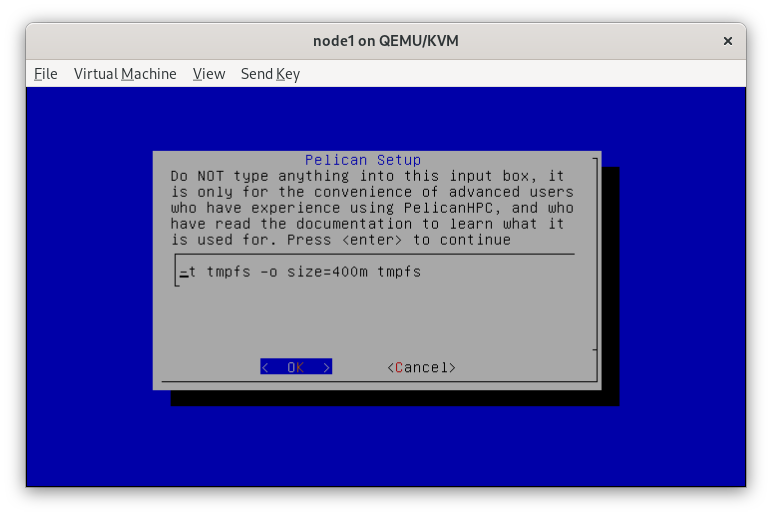
\includegraphics[width=0.7\linewidth]{1-05}
	\caption{Способ загрузки ОС}
	\label{init/05}
\end{figure}

\begin{figure}[H]
	\centering
	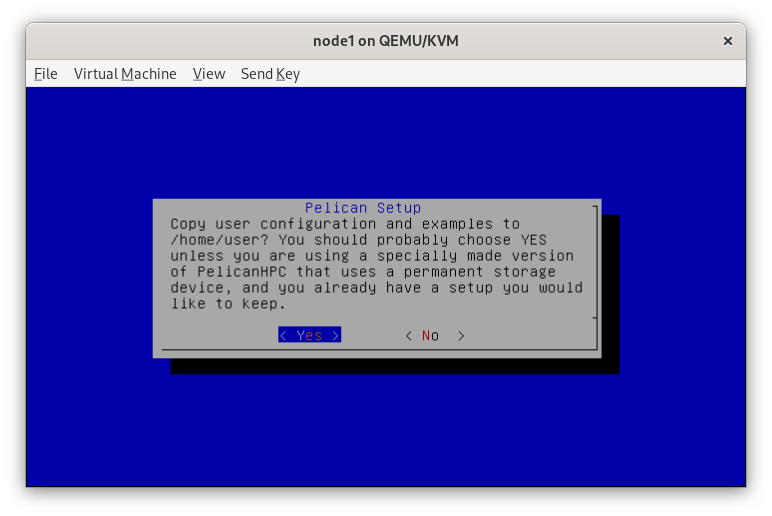
\includegraphics[width=0.7\linewidth]{1-06}
	\caption{Конфигурирование пользователя}
	\label{init/06}
\end{figure}

\begin{figure}[H]
	\centering
	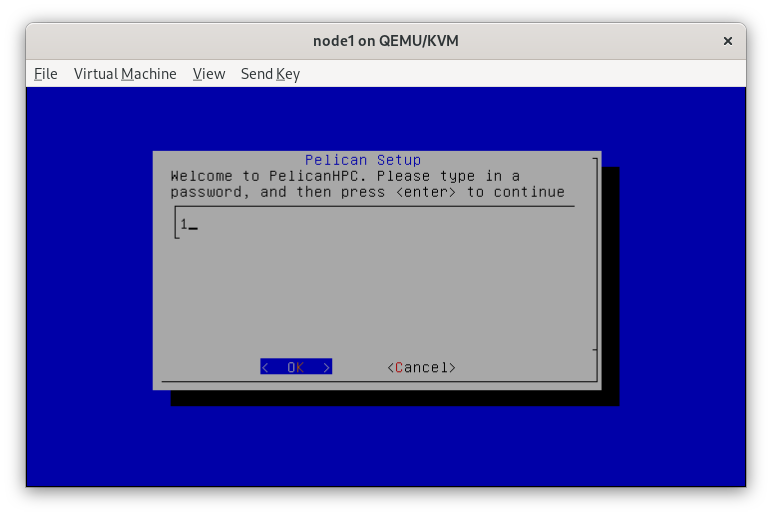
\includegraphics[width=0.7\linewidth]{1-07}
	\caption{Задание пароля пользователя}
	\label{init/07}
\end{figure}

\begin{figure}[H]
	\centering
	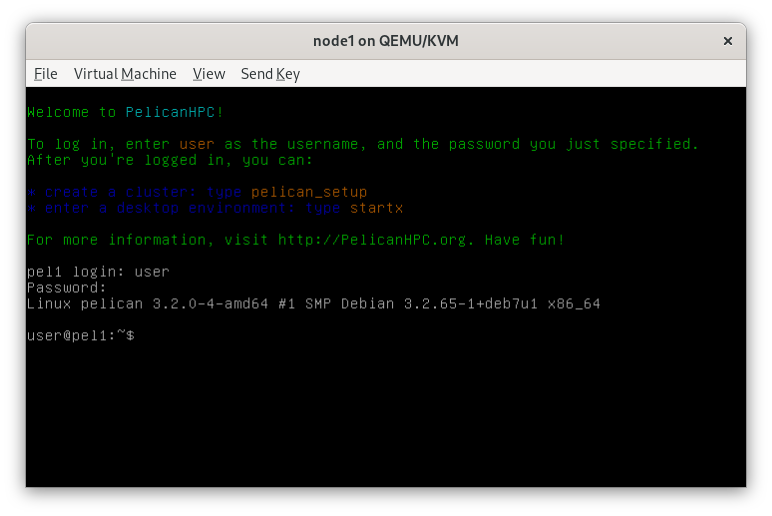
\includegraphics[width=0.7\linewidth]{1-08}
	\caption{Конфигурирование кластера}
	\label{init/08}
\end{figure}

\begin{figure}[H]
	\centering
	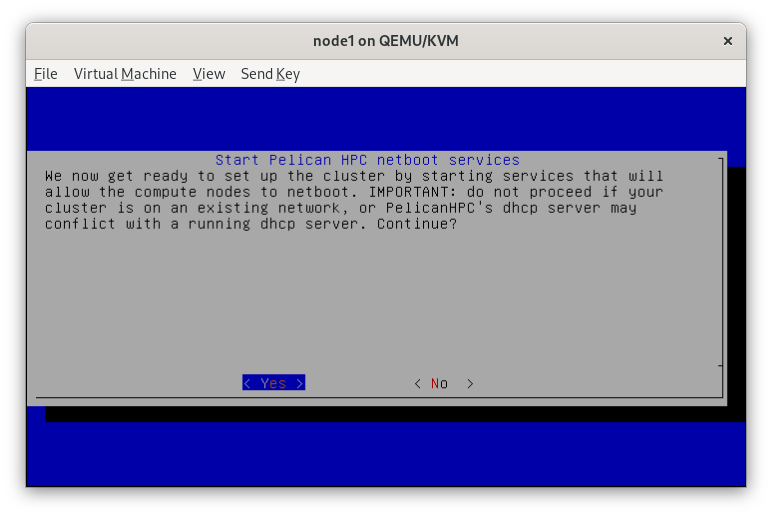
\includegraphics[width=0.7\linewidth]{1-09}
	\caption{Включение сетевого конфигурирование кластера}
	\label{init/09}
\end{figure}

\begin{figure}[H]
	\centering
	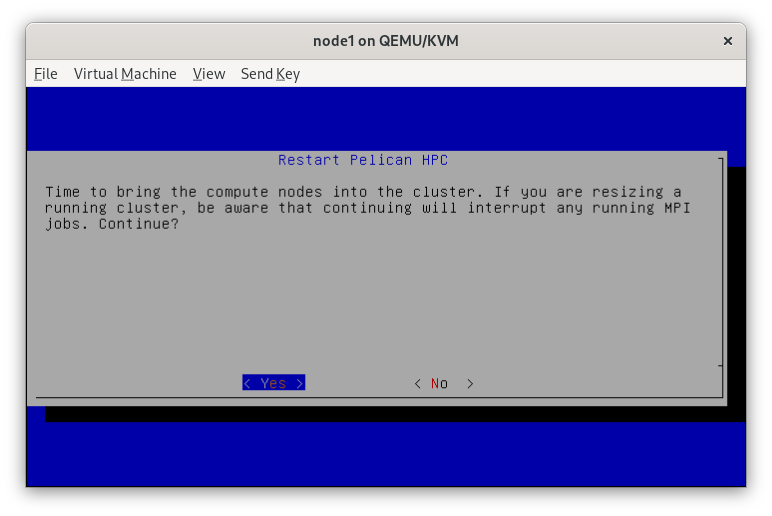
\includegraphics[width=0.7\linewidth]{1-10}
	\caption{Ожидание подключения узлов кластера}
	\label{init/10}
\end{figure}


\subsection{Включение узлов кластера}

Теперь необходимо развернуть узлы кластера. Основное требование к ним --- возможность загрузки ОС по сети. Скриншоты \ref{nodes/01} -- \ref{nodes/07} демострируют конфигурацию одного узла, однако все остальные узлы создаются с такими же параметрами.

\begin{figure}[H]
	\centering
	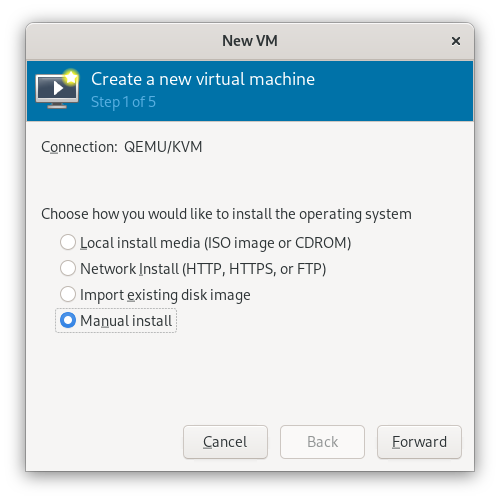
\includegraphics[width=0.5\linewidth]{2-01}
	\caption{Выбор способа установки}
	\label{nodes/01}
\end{figure}

\begin{figure}[H]
	\centering
	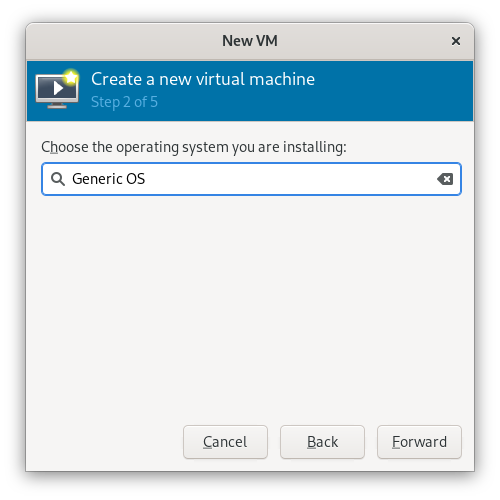
\includegraphics[width=0.5\linewidth]{2-02}
	\caption{Выбор типа образа}
	\label{nodes/02}
\end{figure}

\begin{figure}[H]
	\centering
	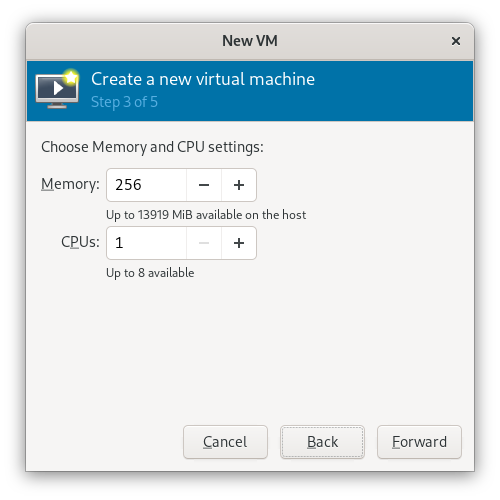
\includegraphics[width=0.5\linewidth]{2-03}
	\caption{Выделение ресурсов узлу}
	\label{nodes/03}
\end{figure}

\begin{figure}[H]
	\centering
	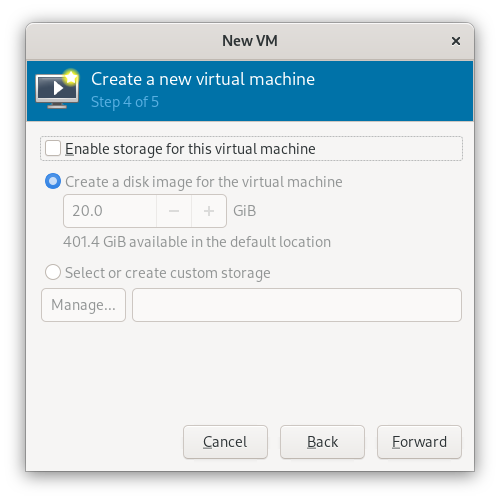
\includegraphics[width=0.5\linewidth]{2-04}
	\caption{Отключение дискового хранилища узла}
	\label{nodes/04}
\end{figure}

\begin{figure}[H]
	\centering
	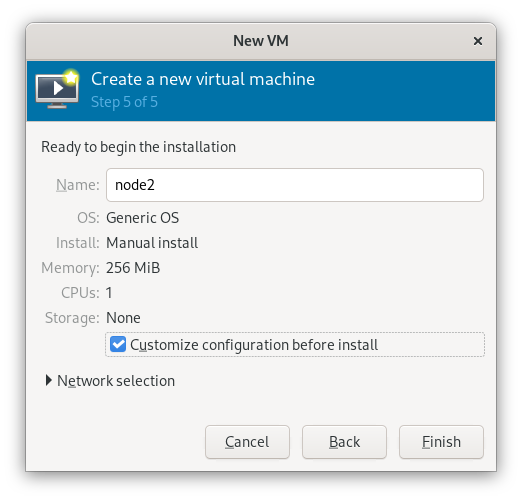
\includegraphics[width=0.5\linewidth]{2-05}
	\caption{Выбор имени узла}
	\label{nodes/05}
\end{figure}

\begin{figure}[H]
	\centering
	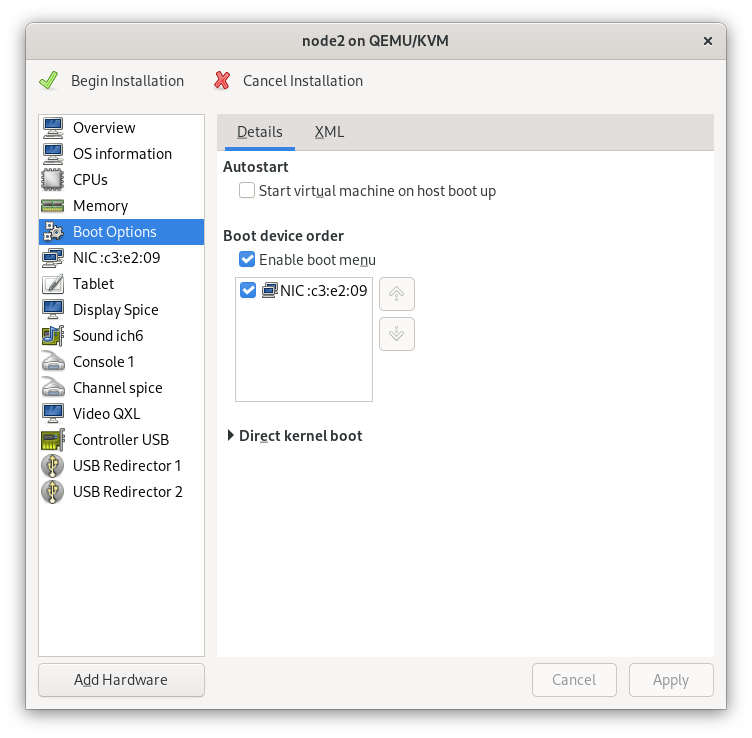
\includegraphics[width=0.7\linewidth]{2-06}
	\caption{Включение сетевой загрузки ОС}
	\label{nodes/06}
\end{figure}

\begin{figure}[H]
	\centering
	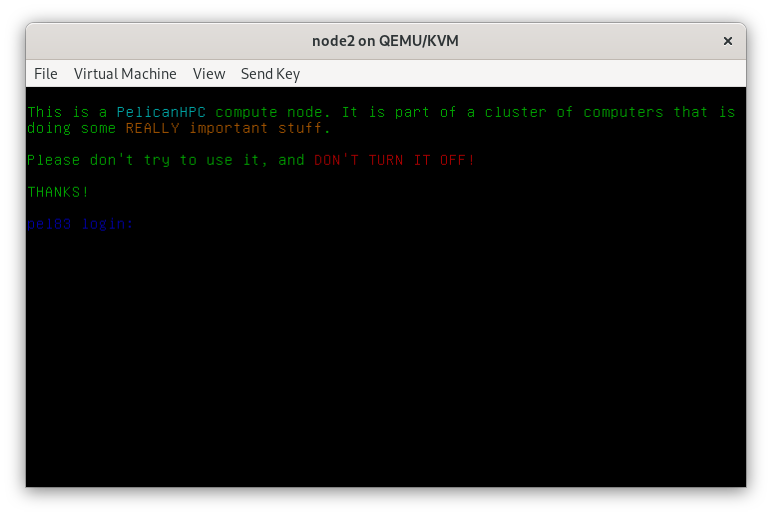
\includegraphics[width=0.7\linewidth]{2-07}
	\caption{Успешная загрузка узла}
	\label{nodes/07}
\end{figure}

\subsection{Донастройка кластера}

После успешного запуска всех узлов кластера нужно выполнить его донастройку. Рисунки \ref{postconf/01} -- \ref{postconf/02} демонстрируют этот процесс.

\begin{figure}[H]
	\centering
	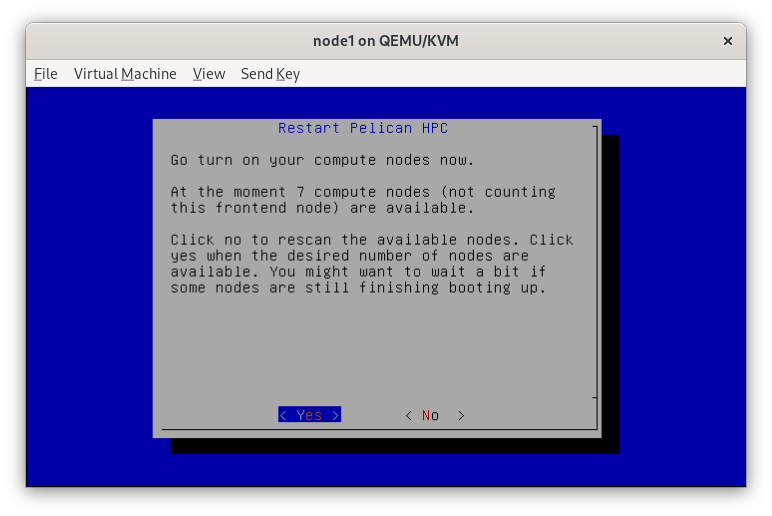
\includegraphics[width=0.7\linewidth]{3-01}
	\caption{Определение количества узлов кластера}
	\label{postconf/01}
\end{figure}

\begin{figure}[H]
	\centering
	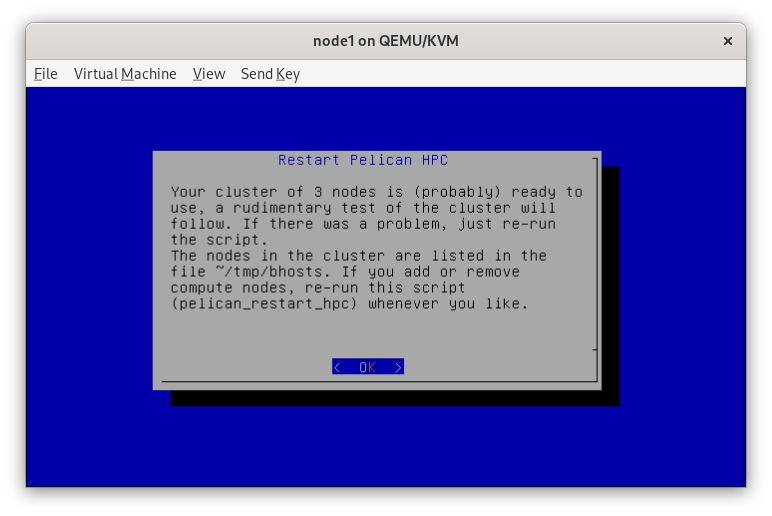
\includegraphics[width=0.7\linewidth]{3-02}
	\caption{Оповещение о готовности кластера}
	\label{postconf/02}
\end{figure}


\section{Тест кластера}
Выполним по 10 тестов для разного количества вычислителей кластера (1 - 8), чтобы получить усредненные значения. Результаты можно посмотреть в таблицах \ref{res/01} -- \ref{res/08}.

\begin{table}[H]
	\caption{Результаты для одного вычислителя}
	\centering
	\begin{tabular}{|c|c|c|}
		\hline
\textbf{№ попытки} & \textbf{Время} & \textbf{MFLOPS} \\ \hline
		1  & 0.61 & 2933 \\ \hline
		2  & 0.61 & 2930 \\ \hline
		3  & 0.63 & 2848 \\ \hline
		4  & 0.63 & 2851 \\ \hline
		5  & 0.62 & 2911 \\ \hline
		6  & 0.62 & 2901 \\ \hline
		7  & 0.63 & 2871 \\ \hline
		8  & 0.61 & 2933 \\ \hline
		9  & 0.61 & 2946 \\ \hline
		10 & 0.62 & 2898 \\ \hline
\textbf{Среднее} & \textbf{0.62} & \textbf{2902} \\
		\hline
	\end{tabular}
	\label{res/01}
\end{table}


\begin{table}[H]
	\caption{Результаты для двух вычислителей}
	\centering
	\begin{tabular}{|c|c|c|}
		\hline
		\textbf{№ попытки} & \textbf{Время} & \textbf{MFLOPS} \\\hline
		1 & 0.33 & 5426 \\ \hline
		2 & 0.31 & 5807 \\ \hline
		3 & 0.34 & 5336 \\ \hline
		4 & 0.34 & 5228 \\ \hline
		5 & 0.33 & 5380 \\ \hline
		6 & 0.32 & 5545 \\ \hline
		7 & 0.33 & 5517 \\ \hline
		8 & 0.32 & 5553 \\ \hline
		9 & 0.32 & 5689 \\ \hline
		10 & 0.33 & 5453 \\ \hline
		\textbf{Среднее} & \textbf{0.33} & \textbf{5493} \\\hline
	\end{tabular}
	\label{res/02}
\end{table}


\begin{table}[H]
	\caption{Результаты для трех вычислителей}
	\centering
	\begin{tabular}{|c|c|c|}
		\hline
		\textbf{№ попытки} & \textbf{Время} & \textbf{MFLOPS} \\\hline
		1 & 0.22 & 8302 \\ \hline
		2 & 0.23 & 7746 \\ \hline
		3 & 0.24 & 7432 \\ \hline
		4 & 0.23 & 7826 \\ \hline
		5 & 0.28 & 6441 \\ \hline
		6 & 0.23 & 7873 \\ \hline
		7 & 0.23 & 7663 \\ \hline
		8 & 0.25 & 7311 \\ \hline
		9 & 0.25 & 7276 \\ \hline
		10 & 0.25 & 7329 \\ \hline
		\textbf{Среднее} & \textbf{0.24} & \textbf{7520} \\\hline
	\end{tabular}
	\label{res/03}
\end{table}


\begin{table}[H]
		\caption{Результаты для четырех вычислителей}
	\centering
	\begin{tabular}{|c|c|c|}
		\hline
		\textbf{№ попытки} & \textbf{Время} & \textbf{MFLOPS} \\\hline
		1 & 0.34 & 5365 \\ \hline
		2 & 0.33 & 5418 \\ \hline
		3 & 0.31 & 5756 \\ \hline
		4 & 0.32 & 5705 \\ \hline
		5 & 0.34 & 5257 \\ \hline
		6 & 0.33 & 5498 \\ \hline
		7 & 0.34 & 5343 \\ \hline
		8 & 0.33 & 5495 \\ \hline
		9 & 0.34 & 5264 \\ \hline
		10 & 0.1833 & 5509 \\ \hline
		\textbf{Среднее} & \textbf{0.33} & \textbf{5461} \\\hline
	\end{tabular}
	\label{res/04}
\end{table}


\begin{table}[H]
	\caption{Результаты для пяти вычислителей}
	\centering
	\begin{tabular}{|c|c|c|}
		\hline
		\textbf{№ попытки} & \textbf{Время} & \textbf{MFLOPS} \\\hline
		1 & 0.28 & 6433 \\ \hline
		2 & 0.29 & 6268 \\ \hline
		3 & 0.27 & 6700 \\ \hline
		4 & 0.27 & 6552 \\ \hline
		5 & 0.27 & 6613 \\ \hline
		6 & 0.27 & 6550 \\ \hline
		7 & 0.27 & 6617 \\ \hline
		8 & 0.26 & 6801 \\ \hline
		9 & 0.27 & 6672 \\ \hline
		10 & 0.27 & 6621 \\ \hline
		\textbf{Среднее} & \textbf{0.27} & \textbf{6583} \\\hline
	\end{tabular}
	\label{res/05}
\end{table}


\begin{table}[H]
	\caption{Результаты для шести вычислителей}
	\centering
	\begin{tabular}{|c|c|c|}
		\hline
		\textbf{№ попытки} & \textbf{Время} & \textbf{MFLOPS} \\\hline
		1 & 0.22 & 8011 \\ \hline
		2 & 0.23 & 7666 \\ \hline
		3 & 0.24 & 7369 \\ \hline
		4 & 0.24 & 7587 \\ \hline
		5 & 0.24 & 7625 \\ \hline
		6 & 0.24 & 7366 \\ \hline
		7 & 0.26 & 6932 \\ \hline
		8 & 0.24 & 7450 \\ \hline
		9 & 0.25 & 7265 \\ \hline
		10 & 0.24 & 7412 \\ \hline
		\textbf{Среднее} & \textbf{0.24} & \textbf{7468} \\\hline
	\end{tabular}
	\label{res/06}
\end{table}


\begin{table}[H]
	\caption{Результаты для семи вычислителей}
	\centering
	\begin{tabular}{|c|c|c|}
		\hline
		\textbf{№ попытки} & \textbf{Время} & \textbf{MFLOPS} \\\hline
		1 & 0.29 & 6210 \\ \hline
		2 & 0.29 & 6115 \\ \hline
		3 & 0.29 & 6214 \\ \hline
		4 & 0.29 & 6272 \\ \hline
		5 & 0.30 & 5928 \\ \hline
		6 & 0.28 & 6377 \\ \hline
		7 & 0.33 & 5482 \\ \hline
		8 & 0.30 & 6063 \\ \hline
		9 & 0.35 & 5191 \\ \hline
		10 & 0.29 & 6281 \\ \hline
		\textbf{Среднее} & \textbf{0.30} & \textbf{6013} \\\hline
	\end{tabular}
	\label{res/07}
\end{table}


\begin{table}[H]
	\caption{Результаты для восьми вычислителей}
	\centering
	\begin{tabular}{|c|c|c|}
		\hline
		\textbf{№ попытки} & \textbf{Время} & \textbf{MFLOPS} \\\hline
		1 & 0.26 & 6914 \\ \hline
		2 & 0.26 & 7038 \\ \hline
		3 & 0.27 & 6624 \\ \hline
		4 & 0.29 & 6302 \\ \hline
		5 & 0.31 & 5734 \\ \hline
		6 & 0.26 & 6989 \\ \hline
		7 & 0.26 & 7043 \\ \hline
		8 & 0.26 & 7023 \\ \hline
		9 & 0.26 & 6996 \\ \hline
		10 & 0.31 & 5716 \\ \hline
		\textbf{Среднее} & \textbf{0.27} & \textbf{6638} \\\hline
	\end{tabular}
	\label{res/08}
\end{table}


Визуализируем полученные результаты в виде графиков. Они продемострированы на рисунках \ref{plot/01} и \ref{plot/02}.


\begin{figure}[H]
	\centering
	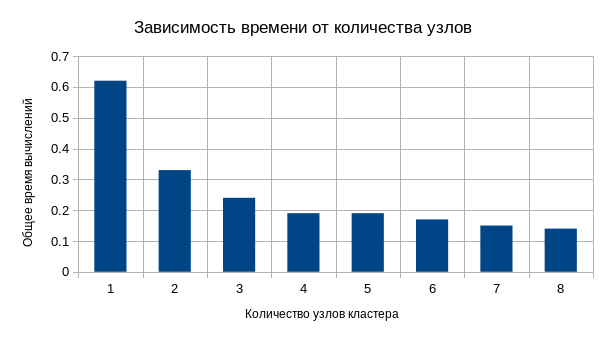
\includegraphics[width=\linewidth]{4-01}
	\caption{График времени}
	\label{plot/01}
\end{figure}


\begin{figure}[H]
	\centering
	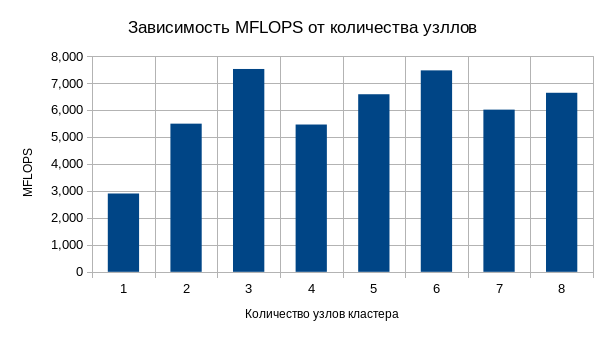
\includegraphics[width=\linewidth]{4-02}
	\caption{График MFLOPS}
	\label{plot/02}
\end{figure}


\section{Анализ полученных результатов}
Исходя из полученных результатов, можно сказать, что с ростом числа вычислителей при недостатке числа узлов количество MFLOPS изменяется циклически. Такое поведение можно объяснить задержками (транспортными и синхронизации) и особенностью вычислительной задачи. Не исключено, что при использовании другой программы будут получены другие результаты.





